%%%%%%%%%%%%%%%%%%%%%%%%%%%%%%%%%%%%%%%%%
% Stylish Article
% LaTeX Template
% Version 2.1 (1/10/15)
%
% This template has been downloaded from:
% http://www.LaTeXTemplates.com
%
% Original author:
% Mathias Legrand (legrand.mathias@gmail.com) 
% With extensive modifications by:
% Vel(vel@latextemplates.com)
%
% License:
% CC BY-NC-SA 3.0 (http://creativecommons.org/licenses/by-nc-sa/3.0/)
%
%%%%%%%%%%%%%%%%%%%%%%%%%%%%%%%%%%%%%%%%%

%----------------------------------------------------------------------------------------
%	PACKAGES AND OTHER DOCUMENT CONFIGURATIONS
%----------------------------------------------------------------------------------------

\documentclass[fleqn,10pt]{JLA_article} % Document font size and equations flushed left

\usepackage[english]{babel} % Specify a different language here - english by default

\usepackage{lipsum} % Required to insert dummy text. To be removed otherwise
\usepackage{hyperref}
\usepackage{graphicx}
\usepackage{subfig}
\usepackage{subcaption} 
\usepackage{amsthm}
\usepackage{amsmath}
\usepackage{float}

%----------------------------------------------------------------------------------------
%	HYPERLINKS
%----------------------------------------------------------------------------------------

\usepackage{hyperref} % Required for hyperlinks
\hypersetup{hidelinks,colorlinks,breaklinks=true,urlcolor=color2,citecolor=color1,linkcolor=color1,bookmarksopen=false,pdftitle={Title},pdfauthor={Author}}

%----------------------------------------------------------------------------------------
%	ARTICLE INFORMATION
%----------------------------------------------------------------------------------------

\PaperTitle{Analyzing Educational Priorities Over Time Using Topic Modeling} % Article title

\Authors{Madison Hobbs\textsuperscript{1}, Evan Liang\textsuperscript{2}, Aanya Alwani\textsuperscript{3}, Jean Selasi Adedze\textsuperscript{4}, Dominique Macias\textsuperscript{5}, Dr. Talithia Williams\textsuperscript{6}} % Authors
\affiliation{\textsuperscript{1}\textit{Department of Mathematics, Harvey Mudd College, Claremont, USA. email icon: mhobbs@g.hmc.edu}} % Author affiliation
\affiliation{\textsuperscript{2}\textit{Department of Mathematics, Harvey Mudd College, Claremont, USA. email icon: eliang@g.hmc.edu}} % Author affiliation
\affiliation{\textsuperscript{3}\textit{Department of Mathematics, Harvey Mudd College, Claremont, USA. email icon: aalwani@g.hmc.edu}} % Author affiliation
\affiliation{\textsuperscript{4}\textit{Department of Mathematics, Harvey Mudd College, Claremont, USA. email icon: sadedze@g.hmc.edu}} % Author affiliation
\affiliation{\textsuperscript{5}\textit{Department of Mathematics, Harvey Mudd College, Claremont, USA. email icon: dmacias@g.hmc.edu}} % Author affiliation
\affiliation{\textsuperscript{6}\textit{Department of Mathematics, Harvey Mudd College, Claremont, USA. email icon: twilliams@g.hmc.edu}} % Author affiliation

% include keywords separated by commas
\Keywords{topic modeling, education, syllabi.} 

\Submitted{mm/dd/yy}
\Accepted{mm/dd/yy}
\Published{mm/dd/yy}

\Volume{x}
\Number{x}
\Pages{1---10}
\Doi{xxx-xxx-xxx}
%----------------------------------------------------------------------------------------
%	NOTES FOR PRACTICE OR RESEARCH
%----------------------------------------------------------------------------------------
\WithoutNotestrue %If this paper does NOT have notes
\Notesname{Notes for Practice} %If this is a Research Paper
%\Notesname{Notes for Research} %If this is a Practitioner Paper


\note{This is an example of a note to practice or research.}
\note{This is a second example of a note to practice or research.}
\note{This is a third example of a note to practice or research.} %Add more notes if necessary

%----------------------------------------------------------------------------------------
%	ABSTRACT
%----------------------------------------------------------------------------------------
%Abstracts shall not exceed 200 words. Do not use a heading for the abstract or headings within the abstract.
\Abstract{\\How can the overarching curriculum of educational institutions be studied over time? We leverage unsupervised topic modeling to analyze a corpus of syllabi spanning 13 years from Oxford College at Emory University. By generating topics and comparing these across the years, we can estimate how much each topic is emphasized in the curriculum of Oxford College at Emory University over time.\\}

%----------------------------------------------------------------------------------------

\begin{document}

\flushbottom % Makes all text pages the same height

\maketitle % Print the title and abstract box

%\tableofcontents % Print the contents section

\thispagestyle{fancy} % Add header to first page


%----------------------------------------------------------------------------------------
%	ARTICLE CONTENTS
%----------------------------------------------------------------------------------------

\section{Introduction} % The \section*{} command stops section numbering

\addcontentsline{toc}{section}{Introduction} % Adds this section to the table of contents

In recent times, topic modeling has emerged as an innovative tool to extract meaningful information from large sources of text. Part of the surge in attention to topic modeling lies in its ability to uncover insights from documents that would otherwise never be hard to discern in aggregate by a human. As educational institutions increasingly adopt data driven approaches in their administrative practices, we see immense potential in leveraging topic modeling techniques to extract insights from large collection of documents like written work, handbooks, syllabi, course evaluations, textbooks among others that are abundant in these institutions.

In this paper, we analyze the changes in the school curriculum over time. We leverage topic modeling to analyze a corpus of syllabi spanning 13 years from Oxford College at Emory University. By generating topics and comparing these across the years, we can estimate how much each topic is emphasized in the curriculum of Oxford College at Emory University over time. This type of analysis has the potential to inform parents, policy makers and school administrator of how priorities of educational institutions have changed in time.  





%This is example text. Note that JLA uses up to 3 levels of headings (e.g. 1., 1.1, 1.1.1). Please do not add additional levels beyond the three that have been provided. This is an example of including math $\cos\pi=-1$ and $\alpha$ directly within the text\footnote{And an example of a footnote including math $\cos\pi=-1$ and $\alpha$ in the text.}. Important formulas should be presented on a seperate line as shown in the next section (See Formula 1). All figures and tables should be explicitly referenced in the appropriate part of the text (See Table 1 and Figure 2).

%This template use the  \href{http://ctan.uniminuto.edu/biblio/bibtex/contrib/apacite/apacite.pdf}{apacite package}. This is an example on how to cite \cite{GloVe}.  

%------------------------------------------------

\section{Related Work}

Sekiya et al. present a similar investigation to ours with a slightly different angle \cite{8190598}. Rather than looking at all course subjects across time at one school, they narrow the focus to computer science curriculum across multiple schools within the same time frame. Furthermore, rather than having to train a topic model themselves, they leverage the pre-existing CS2013 Body of Knowledge (BOK), produced by the ACM and IEEE Computer Society and detailing the 18 primary topics in Computer Science curriculum as of 2013. Sekiya et al. used those 18 topics to train a simplified, supervised Latent Dirichlet Allocation model (ssLDA) which then outputs, for a given unseen computer science syllabus, how much each of those 18 core topics were represented. However, since we lack predefined topics, our work involves training unsupervised topic models to discover the core topics across all disciplines and observe how these have changed over an 13 year period at Oxford College of Emory University. 

Another publication more similar to our temporal analysis though not using syllabi is ``Studying the History of Ideas Using Topic Models" \cite{hall08}. Like us, they have time series data; in their case, journal publications from the ACL Anthology (a compilation of natural language processing papers) spanning multiple years. Also like us, they train a single topic model on their entire corpus, spanning all years. Unlike us, they have 12,500 documents compared to our 3,778. They also only mention trying one algorithm on a fixed number of topics (100 topics with LDA), whereas we select a best model across multiple algorithms and numbers of topics. After training a model, Hall et al. hand-select a subset of the topics with which to proceed, then observe the prevalence of those topics for documents from each year. This technique inspired the way we approach the temporal analysis in our paper. 

%------------------------------------------------

\section{Methods}

\subsection{Data}
Our dataset consists of 3,778 syllabi from Oxford College of Emory University from 2001 to 2014. This was the largest and most temporally expansive collection of syllabi we could find on a university website for scraping. After scraping syllabi from Oxford's \href{https://app.oxford.emory.edu/WebApps/Directories/EResources/index.cfm}{website}, we discarded syllabi which were scanned copies because text could not be easily extracted in such format. This explains why we consider syllabi from 2001 to present even though Oxford College has syllabi from 1990.
\subsection{Processing}
First, we use regular expressions to extract words composed of letters from the English alphabet. For consistent representation, we convert all words to lower-case. In order to improve the effectiveness of topic modeling algorithms, we remove stop words such as ``the", ``a", ``he", etc using NLTK's pre-defined list of stop words  \cite{Loper02nltk:the}. Using NLTK again, we further filter out words not in the English language. Finally, we use TF-IDF from the Scikit-learn package in Python \cite{Pedregosa} to filter out any other words which do not provide differentiable course-related information for topic modeling algorithms to leverage. 

\subsection{Topic Modeling}
Topic modeling is an unsupervised learning algorithm that takes in a large corpus of text data and returns a specified number of representative topics found in the corpus. A topic is defined as probability distribution over fixed vocabulary. Words in a topic are sorted in descending order using the probability assigned to each word in the topic. The top $k$ words in a topic (for some $k$ defined by the user) reflect the overarching and related concepts of the topic. Topic modeling therefore provides a method of extracting insights about the high level meaning of a text. 
An example of an output of topic modelling is shown in figure \ref{fig:distribution}.
\begin{figure}[H]
    \centering
    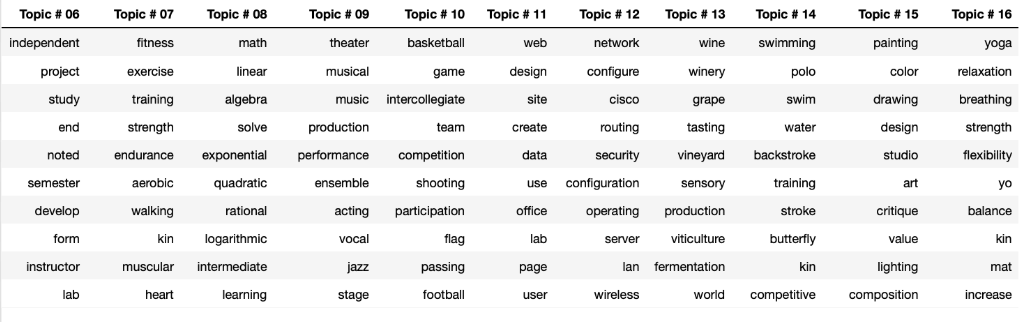
\includegraphics[scale=0.5]{topic-distribution.png}
    \caption{Example distribution of topics output by a trained topic model}
    \label{fig:distribution}
\end{figure}
We considered two well-known methods methods for topic modeling: Latent Dirichlet Allocation and Non-negative Matrix Factorization.

\subsubsection{Non-negative Matrix Factorization}

The first method employed uses a novel interpretation of low-rank approximation of matrices. The Non-negative Matrix Factorization (NMF for short) method takes in a bag-of-words $n\times m$ matrix $A$ whose entry $A_{ij}$ is the number of occurrences of word $j$ in document $i$. NMF seeks to find the closest approximation of $A$ as a product of a $n\times k$ matrix $W$ and a $k\times m$ matrix $H$ with the condition that all entries of $W$ and $H$ are non-negative. In other words, NMF outputs $W,H$ with the prescribed dimensions such that $\|A-WH\|_F$ is minimized.

To interpret the output matrices $W$ and $H$, we call $W$ the \textit{basis matrix} and $H$ the \textit{coefficient matrix}. The prescribed number $k$ here represents the number of topics we wish to extract from the text. To find out the top words are associated with the $i$-th topic, we examine the $i$-th row of the $H$ matrix and take the words whose position in that row has a high value. In other words, the entry $H_{ij}$ measures how relevant word $j$ is for topic $i$. Next, if we want to find out what topics are the most prevalent in the $i$-th corpus document, we examine the $i$-th row of the $W$ matrix and take the topics whose position in that row has a high value. Although there are methods to perform this task with unseen documents that were not used in training, we omit their discussions here as they were not used for our experiments.

\subsubsection{Latent Dirichlet Allocation}

Latent Dirichlet Allocation, commonly known as LDA, is a generative probabilistic model that prescribes each document in a corpus with a finite mixture of topics from an underlying topic distribution. LDA views each document in a corpus as a generated item from a collection in order to infer the topic distribution. The generative process that LDA uses to infer the underlying topic distribution represents the topic distribution $\theta_m$ for each document $m$ as a random variable from a Dirichlet distribution with sparse priors, where each topic is a distribution over all of the words. For each of $N$ words in document $m$, a topic $z_n \sim \text{Multinomial}(\theta)$ is chosen and a word $w_n$ is chosen from a multinomial distribution conditioned on $z_n$. LDA requires the modeller to input number of topics. In our experiments, we built our LDA models from LdaModel in the Python \texttt{gensim} package. 

% http://www.jmlr.org/papers/volume3/blei03a/blei03a.pdf
% see this: https://medium.com/@lettier/how-does-lda-work-ill-explain-using-emoji-108abf40fa7d


\subsection{Training \& Selecting Topics}

We first train both LDA and NMF models on all Oxford College syllabi from 2001 to 2014 with various numbers of topics (50, 100, 150, and 200). Within LDA and NMF each, we compare the topics generated and select the best model by plotting and manual inspection of the topics. Then, comparing our best models from both NMF and LDA we determine which model outperforms the other. From this best model, we hand-select 43 topics with which to proceed in our analysis.

\subsection{Assessing Change Through Time}

We aim to assess the changes in courses offered over time using the topic model. To do so, we classify a syllabus by the topic that yields the highest relevance over the hand-selected topics. This is possible due to the topic distribution feature both techniques possess. For each year, we assess what proportion of syllabi was most related to each topic. In the next section, we will present graphs of these analysis as well as the hand-selected topics.  

%------------------------------------------------

\section{Results and Discussion}

\subsection{Selected Model}

After comparing topic coherence and manually observing the topics output by LDA and NMF for 50, 100, 150, and 200 topics, we decided that NMF with 100 topics gave the best results. Even the best LDA model gave much worse topics than NMF which is surprising since LDA is often the model more preferred in literature (as was the case with both \cite{hall08} and \cite{8190598}). However, on small and sparse corpuses, NMF does as well and oftentimes better than LDA as shown by \cite{chen_zhang_liu_ye_lin_2019}. For this reason, it is perfectly reasonable that NMF was more successful in our task of under 4,000 one-to-two-page syllabi.

%Displayed below is a comparison of a random sample of 10 LDA topics

%\begin{figure}[H]
  %  \centering
   % \includegraphics[scale=0.6] %{jla-template/lda_bad_topics.png}
  %  \caption{Random sample of 10 LDA topics generated from a 100-topic LDA model}
  %  \label{fig:my_label}
%\end{figure}

%\begin{figure}[H]
   % \centering
   % 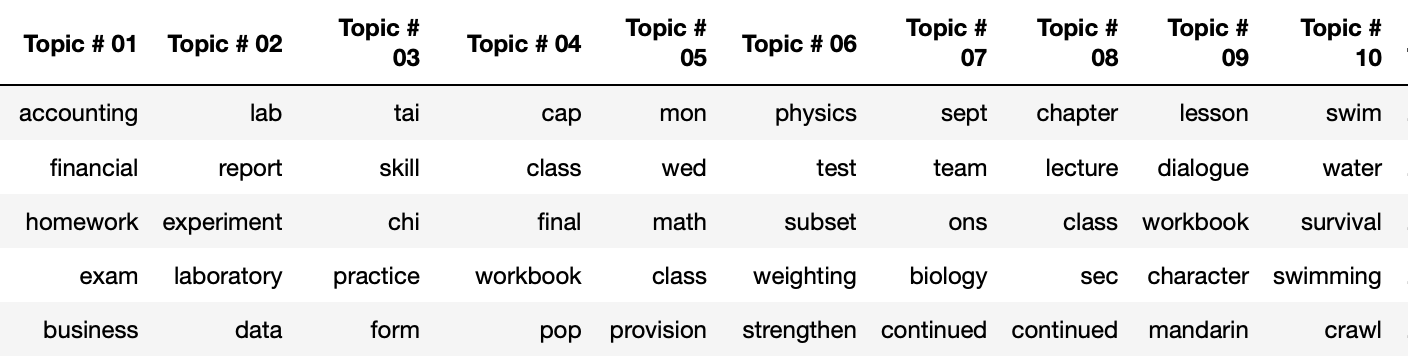
\includegraphics[scale=0.7] {jla-template/nmf_topics_sample.png}
    %\caption{Random sample of 10 LDA topics generated from a %100-topic LDA model}
   % \label{fig:my_label}
%\end{figure}

\subsection{Selected Topics}

The hand-selected 43 topics are displayed in the table below.

\begin{center}
    \begin{tabular}{ |c|c|c|c|c|c| } 
        \hline
        \textbf{Topic Description} & \textbf{Word 1} & \textbf{Word 2} & \textbf{Word 3} & \textbf{Word 4} & \textbf{Word 5} \\
        \hline
        \textbf{Anatomy} & dissection & lab & physiology & anatomy & laboratory \\
        \hline
        \textbf{Anthropology} & anthropology & park & culture & cultural & archaeology \\
        \hline
        \textbf{Art} & studio & drawing & color & charcoal & art \\
        \hline
        \textbf{Astronomy} & laboratory & astronomy & observation & universe & heavens \\
        \hline
        \textbf{Biology} & biology & lab & genetics & laboratory & scientific \\
        \hline
        \textbf{Botany} & field & plant & woody & trip & identification \\
        \hline
        \textbf{Child Development} & development & child & discussion & childhood & group \\
        \hline
        \textbf{Classical Studies} & metamorphoses & homer & myth & mythology & tragedy \\
        \hline
        \textbf{Dance} & dance & ballroom & folk & cha & cultural \\
        \hline
        \textbf{Economics} & economic & march & policy & demand & market \\
        \hline
        \textbf{Environmental Science} & environmental & ozone & lab & stream & science \\
        \hline
        \textbf{Ethics} & ethics & ethical & morals & utilitarianism & philosophy \\
        \hline
        \textbf{Finance} & accounting & financial & business & time & assets \\
        \hline
        \textbf{French} & sur & pour & dissertation & reprise & lire \\
        \hline
        \textbf{Geology} & geology & earth & lab & laboratory & geologic \\
        \hline
        \textbf{German} & mitt & german & thema & die & sie \\
        \hline
        \textbf{Gerontology} & aging & aged & dying & death & surrounding \\
        \hline
        \textbf{Golf} & golf & game & score & chipping & swing \\
        \hline
        \textbf{Health} & fitness & activity & physical & training & running \\
        \hline
        \textbf{Linear Algebra} & linear & algebra & differential & matrices & problem \\
        \hline
        \textbf{Literature} & fiction & poetry & portfolio & short & march \\
        \hline
        \textbf{Logic} & logic & reasoning & categorical & syllogism & ordinary \\
        \hline
        \textbf{Mandarin Chinese} & dialogue & workbook & character & mandarin & cheng \\
        \hline
        \textbf{Martial Arts} & tai & skill & chi & practice & form \\
        \hline
        \textbf{Mathematics} & gateway & calculus & trigonometric & derivative & logarithmic  \\
        \hline
        \textbf{Media Studies} & screening & film & cinema & reserve & sound \\
        \hline
        \textbf{Meteorology} & lab & weather & climate & meteorology & atmospheric \\
        \hline
        \textbf{Music Education} & music & musical & western & concert & classical \\
        \hline
        \textbf{Musical Performance} & dress & rehearsal & black & concert & music \\
        \hline
        \textbf{Philosophy} & philosophy & philosophical & philosopher & reverse & ken \\
        \hline
        \textbf{Physical Education} & cycling & fitness & indoor & workout & physical \\
        \hline
        \textbf{Poetry} & poetry & workshop & mid & poem & story\\
        \hline
        \textbf{Political Philosophy} & republic & utopia & book & political & politics \\
        \hline
        \textbf{Political Science} & politics & political & science & syllabus & international\\
        \hline
        \textbf{Probability and Statistics} & statistics & statistical & probability & data & hypothesis \\
        \hline
        \textbf{Proofs} & mathematics & theory & mathematical & landau & analysis \\
        \hline
        \textbf{Racket Sports} & singles & play & smash & badminton & net \\
        \hline
        \textbf{Spanish} & leer & lunes & antes & para & las  \\
        \hline
        \textbf{Swimming} & pool & swim & swimming & water & underwater \\
        \hline
        \textbf{Theater} & theater & play & theatrical & performance & production \\
        \hline
        \textbf{US Government and Politics} & political & federalist & march & federalism & bureaucracy \\
        \hline
        \textbf{Weight Training} & lift & weight & training & fitness & muscle \\
        \hline
        \textbf{Western History} & art & ancient & architecture & paleolithic & aesthetic \\
        \hline
    \end{tabular}
\end{center}

\subsection{Historical Trends in Emory University Courses}

We now present some plots of syllabus frequency over time. Specifically, we examine examples of topics that increase or decrease in prevalence. Due to the anomalous nature of the number of syllabi in recent years, we will restrict the time of observation from 2001 to 2014. To visualize the trend of a selected topic, we plot the proportion of syllabi that are best represented by that topic.


\subsubsection{Topics Increasing in Prevalence}

We see an increase in relative frequency of syllabi that are best represented by the \textit{Biology} and \text{Mandarin Chinese} topics. Both observations could be explained by their emerging popularity as subjects. For example, more people might be realizing that Mandarin is a useful language to learn as it is spoken by many people.

\begin{figure}[H]
\centering
    \begin{subfigure}
    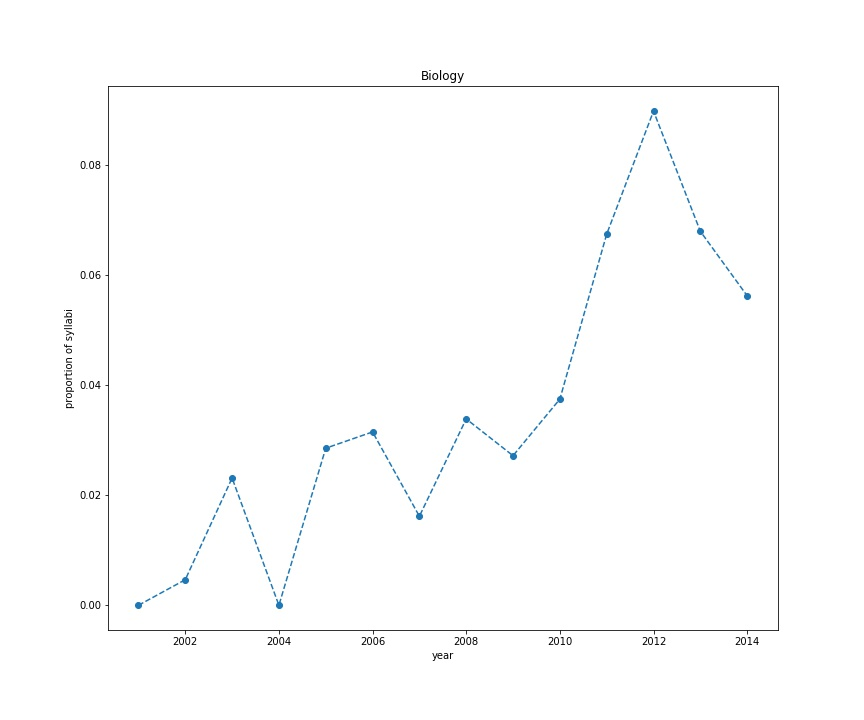
\includegraphics[scale=0.4] {jla-template/biology_plot.jpg}
   \caption{This plot displays the relative frequency of syllabi that are best represented by the \textit{Biology} topic between 2001 and 2014.}
    \end{subfigure}
    %
    \begin{subfigure}
    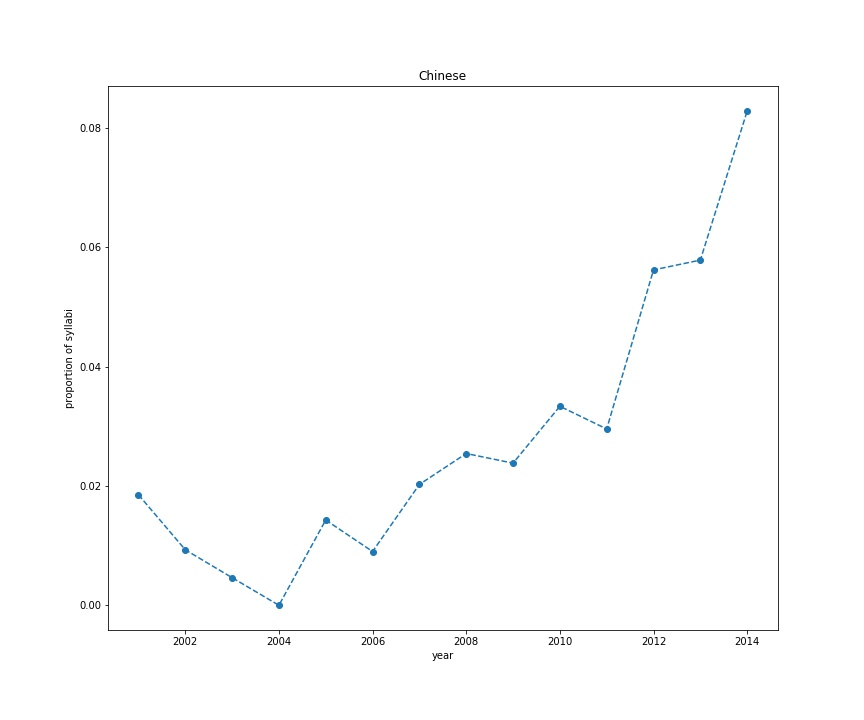
\includegraphics[scale=0.4] {jla-template/chinese_plot.jpg}
   \caption{This plot displays the relative frequency of syllabi that are best represented by the \textit{Mandarin Chinese} topic between 2001 and 2014.}
    \end{subfigure}
\end{figure}




\subsubsection{Topics Diminishing in Prevalence}

\begin{figure}[H]

    \begin{subfigure}
    \centering
    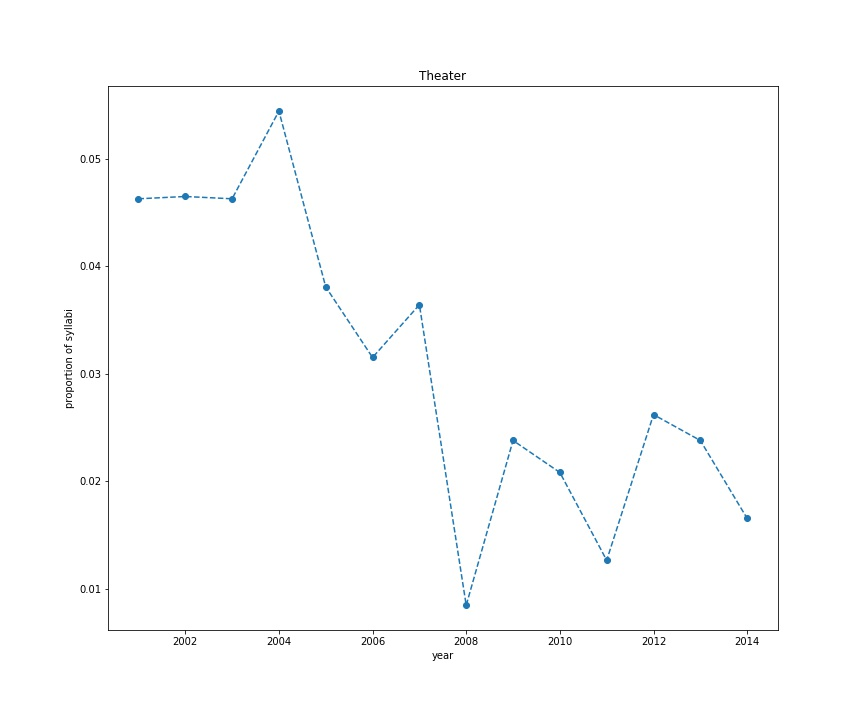
\includegraphics[scale=0.4] {jla-template/theater_plot.jpg}
    \caption{This plot displays the relative frequency of syllabi that are best represented by the \textit{Theater} topic between 2001 and 2014.}
    \label{fig:my_label}
    \end{subfigure}
    %
    \begin{subfigure}
    \centering
    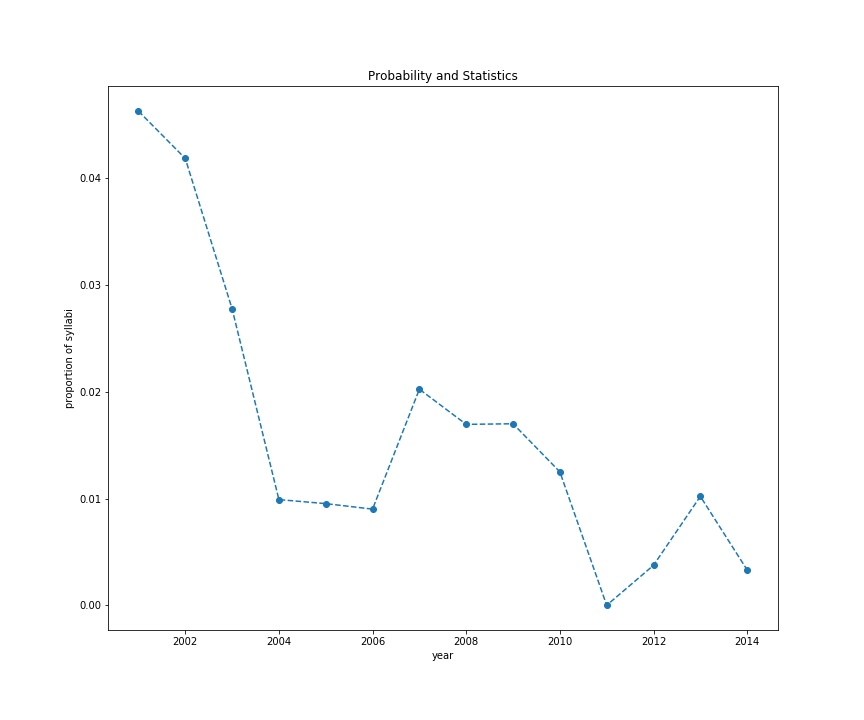
\includegraphics[scale=0.4] {jla-template/stats_plot.jpg}
    \caption{This plot displays the relative frequency of syllabi that are best represented by the \textit{Probability and Statistics} topic between 2001 and 2014.}
    \label{fig:my_label}
    \end{subfigure}
\end{figure}

\section{Conclusion}

\subsection{Remarks}

Our research demonstrates the power of topic modeling to uncover the priorities in a university over time. At Oxford College of Emory University, we discover that certain subjects like Biology and Mandarin Chinese have increased in prevalence and certain subjects like Theater and Probability and Statistics have decreased in prevalence between 2001 and 2014.

\subsection{Future Work} 

As our research presented in this paper figures into one part of a larger project with various other stakeholders and other priorities, we were under significant time constraints. As such, our choice of university was influenced by finding a public website we could easily web-scrape which also contained at least 10 years of syllabi. Although it would have been ideal to have had a larger corpus, our work establishes a reproducible pipeline which, upon acquiring more data from a source like the Open Syllabus Project, we would be able to compare multiple universities across time. 

It would be interesting to perform the same type of analysis on a university offering thousands, rather than hundreds, of courses each year. It would also be fascinating to compare the syllabi of private and public universities, or even high schools to community colleges. Finally, Hall et al. were able to compare the papers from three Natural Language Processing conferences over time. Similarly, we could compare three or more universities over the same time frame. We were challenged to find comparable corpuses of syllabi freely available online, but with access to the Open Syllabus Project, this endeavor would be very feasible.

Another idea we discussed, though veered away from due to time limitations and sample size concerns, is analyzing how one course subject (such as literature, statistics, engineering, etc.) changes over time within a single school or across institutions. Say, for example, we focused on statistics. We could then train a topic model on a corpus of syllabi from only statistics courses and generate a number of topics from within statistics. Or, inspired by the work of Sekiya et al., we could find some pre-defined curriculum topics established an educational institution and use classify syllabi based on these topics. Expanding beyond the work of Sekiya et al., we could analyze how statistics courses have changed over time within a single institution or across a sample of universities across the country. 

%------------------------------------------------
\phantomsection
\section*{Acknowledgments} % The \section*{} command stops section numbering
\addcontentsline{toc}{section}{Acknowledgments} % Adds this section to the table of contents

We greatly appreciate Derick Lee, the PilotCity local team, Dr. Talithia Williams, Dr. Weiqing Gu, and the Institute of Education Sciences for supporting our project.

\section*{Declaration of Conflicting Interest} % The \section*{} command stops section numbering

\addcontentsline{toc}{section}{Declaration of Conflicting Interest} % Adds this section to the table of contents

The authors declared no potential conflicts of interest with respect to the research, authorship, and/or publication of this article.

\section*{Funding} % The \section*{} command stops section numbering

\addcontentsline{toc}{section}{Funding} % Adds this section to the table of contents

This study was financially supported by The Institute of Education Sciences.

%----------------------------------------------------------------------------------------
%	REFERENCE LIST
%----------------------------------------------------------------------------------------
\phantomsection
\bibliography{sample}
\nocite{*}

%----------------------------------------------------------------------------------------

\end{document}